\subsubsection{Panel comparativo de Tasa de crecimiento y el Consumo de energ�a}

En la figura ~\ref{fig:TasaDeCrecimientoVsConsumoDeEnergia} se presenta un panel comparativo entre la tasa de crecimiento de clientes y consumo de energ�a. Tambi�n se cuenta con un mapa para filtrar por regi�n del pa�s. 

\textsc{\begin{figure}[H]
	\centering
	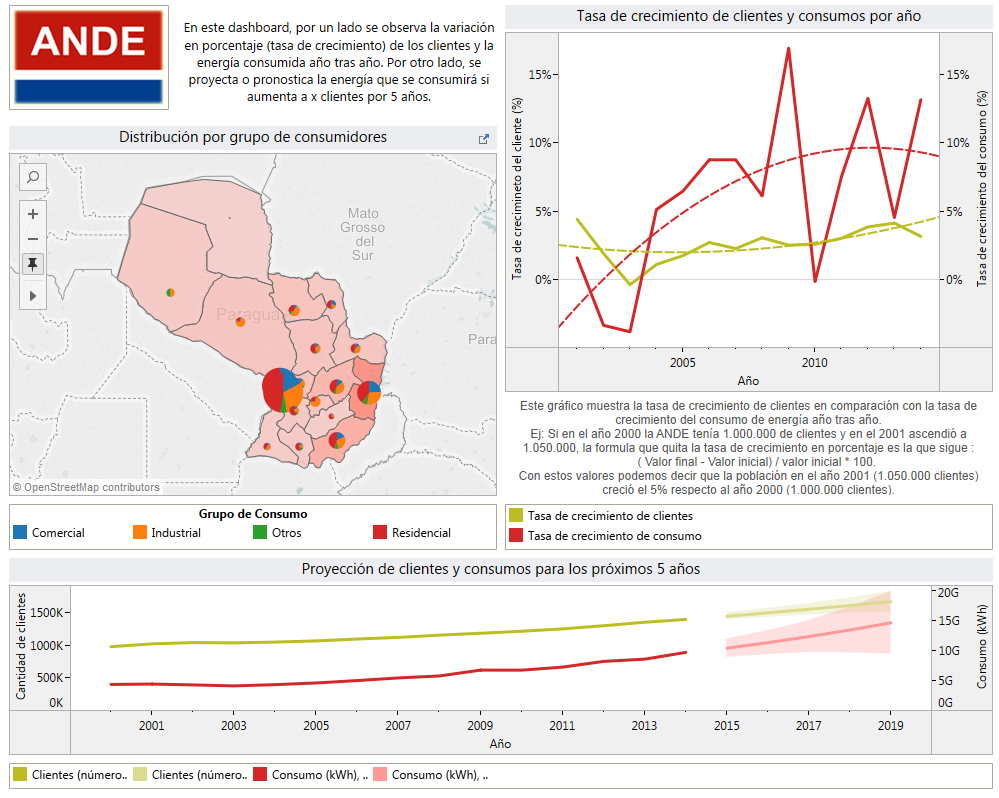
\includegraphics[width=\linewidth]{figuras/TasaDeCrecimientoVsConsumoDeEnergia}
	\caption{Tasa de crecimiento vs Consumo de energ�a}
	\label{fig:TasaDeCrecimientoVsConsumoDeEnergia}
\end{figure}}

En el gr�fico situado a la derecha del mapa (Figura ~\ref{fig:TasaDeCrecimientoVsConsumoDeEnergia2}), se tiene el consumo y crecimiento de clientes. Para un mejor analisis fue necesario suavizar los datos calculando lineas de tendencia, debido a una inestabilidad de los datos de consumo. As� se puede apreciar, que existe una tendencia de crecimiento sostenido durante el tiempo de clientes. Sin embargo, la tendencia que el consumo crezca es mayor al de clientes.

\textsc{\begin{figure}[H]
	\centering
	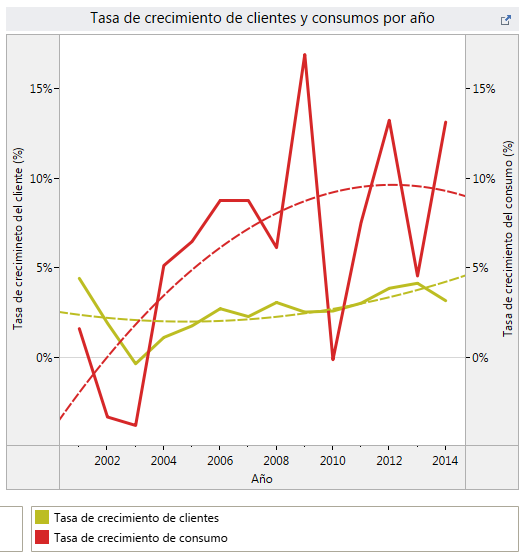
\includegraphics[width=\linewidth]{figuras/TasaDeCrecimientoVsConsumoDeEnergia2}
	\caption{Tasa de crecimiento vs Consumo de energ�a, filtrado por el departamento Alto Paran�}
	\label{fig:TasaDeCrecimientoVsConsumoDeEnergia2}
\end{figure}}

Debajo se presenta un cuadro con la l�nea de cada valor (Figura ~\ref{fig:ProyeccionDeClientesYConsumosParaLosProximos5Anos}), de crecimiento y consumo. Con el uso de un recurso disponible que cuenta la herramienta escogida Tableau, es posible realizar an�lisis predictivo  (forecasting) del crecimiento y consumo. Tableau utiliza un algoritmo llamado Suavizado Exponencial, muy conocido en el �rea de Matem�ticas Estad�sticas. En este gr�fico se puede notar que existe una mayor probabilidad que en los pr�ximos a�os aumente considerablemente el consumo, superando su media. Sin embargo, se nota que el ritmo de crecimiento de clientes es sostenible, y no tiene una alta probabilidad de sufrir un aumento abrupto.

\textsc{\begin{figure}[H]
		\centering
		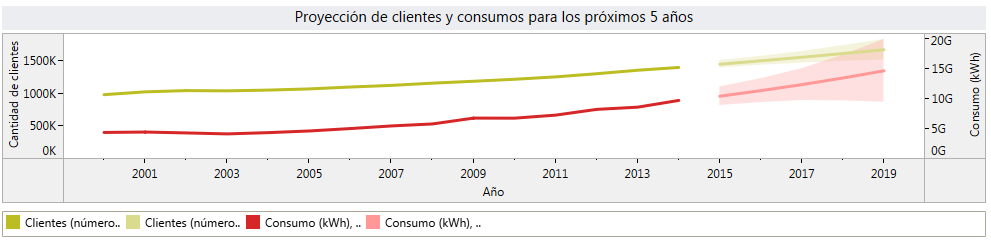
\includegraphics[width=\linewidth]{figuras/ProyeccionDeClientesYConsumosParaLosProximos5Anos}
		\caption{Proyecci�n de clientes y consumos para los pr�ximos 5 a�os}
		\label{fig:ProyeccionDeClientesYConsumosParaLosProximos5Anos}
	\end{figure}}
	